\documentclass[11pt,a4paper]{scrartcl}
\usepackage[T1]{fontenc}
\usepackage[utf8]{inputenc}
%\usepackage[ngerman]{babel}
\usepackage[ngerman,english]{babel}
\selectlanguage{english}
\usepackage{microtype}
\usepackage{lmodern}
\usepackage{amsmath}
\usepackage{amsfonts}
\usepackage{amssymb}
\usepackage{enumerate}
\usepackage{graphicx}
\usepackage{listings}
\usepackage{color}
\usepackage{url}
\usepackage{multicol}
\usepackage{wrapfig}
\usepackage{amsmath}
\usepackage{tikz}
\usetikzlibrary{arrows}


\begin{document}

\author{Ralf Vogler}
\title{Program Optimization}
\subtitle{Exercise sheet 7}

\maketitle

\section*{Exercise 1: Partitioning alias analysis}
\subsection*{1. Analysis}
Partitions:\\
\begin{tabular}{|c|c|}
\hline
 & \{a\}, \{xs\}, \{ys\}, \{t\}, \{a[]\}, \{xs[]\}, \{ys[]\}\\
\hline
(6, 7) & \{a\}, \{xs\}, \{ys\}, \{t, a[]\}, \{xs[]\}, \{ys[]\} \\
(7, 8) & \{a\}, \{xs\}, \{ys\}, \{t, a[], xs[]\}, \{ys[]\} \\
(9, 10) & \{a\}, \{xs\}, \{ys\}, \{t, a[], xs[], ys[]\} \\
\hline
\end{tabular}

\subsection*{2. Second load from a[i] superfluous}
The second load is superfluous for the analysis because in point 8 t and a[] are already in the same partition.
Semantically it is superfluous because the index is also the same.


\section*{Exercise 2: Worklist iteration}
\begin{tabular}{|c|c|}
\multicolumn{2}{c}{Influence sets}\\
\hline
 & \textit{I}\\
\hline
$x_1$ & $\{x_2\}$ \\
$x_2$ & $\{x_1, x_4\}$ \\
$x_3$ & $\{x_2\}$ \\
$x_4$ & $\{x_3\}$ \\
\hline
\end{tabular}
\begin{tabular}{|c|c|c|c||c|}
\multicolumn{5}{c}{Iterations}\\
\hline
D[$x_1$] & D[$x_2$] & D[$x_3$] & D[$x_4$] & W \\
\hline
$\emptyset$ & $\emptyset$ & $\emptyset$ & $\emptyset$ & $x_1, x_2, x_3, x_4$ \\
$\{3\}$ & $\emptyset$ & $\emptyset$ & $\emptyset$ & $x_2, x_3, x_4$ \\
$\{3\}$ & $\{3, 4\}$ & $\emptyset$ & $\emptyset$ & $x_1, x_3, x_4$ \\
$\{3, 4\}$ & $\{3, 4\}$ & $\emptyset$ & $\emptyset$ & $x_2, x_3, x_4$ \\
$\{3, 4\}$ & $\{3, 4\}$ & $\emptyset$ & $\emptyset$ & $x_3, x_4$ \\
$\{3, 4\}$ & $\{3, 4\}$ & $\{1\}$ & $\emptyset$ & $x_2, x_4$ \\
$\{3, 4\}$ & $\{1, 3, 4\}$ & $\{1\}$ & $\emptyset$ & $x_1, x_4$ \\
$\{3, 4\}$ & $\{1, 3, 4\}$ & $\{1\}$ & $\emptyset$ & $x_4$ \\
$\{3, 4\}$ & $\{1, 3, 4\}$ & $\{1\}$ & $\{2, 3, 4\}$ & $x_3$ \\
$\{3, 4\}$ & $\{1, 3, 4\}$ & $\{1, 2, 3\}$ & $\{2, 3, 4\}$ & $x_2$ \\
$\{3, 4\}$ & $\{1, 3, 4\}$ & $\{1, 2, 3\}$ & $\{2, 3, 4\}$ & $[]$ \\
\hline
\end{tabular}


\section*{Exercise 3: Eliminating Partial Redundancies}
\subsection*{1. Analysis}
\begin{tabular}{|c|c|c|}
\hline
& $\mathcal{A}$ & $\mathcal{B}$\\
\hline
1 & $\emptyset$ & $\emptyset$ \\
2 & $\emptyset$ & $\{b+1\}$ \\
4 & $\emptyset$ & $\{a+1\}$ \\
5 & $\{a+1\}$ & $\{a+b\}$ \\
3 & $\{b+1\} \cap \{a+1, a+b\} = \emptyset$ & $\{a+b\}$ \\
6 & $\{a+b\}$ & $\emptyset$ \\
\hline
\end{tabular}

\subsection*{2. Transformations}
Original:\\
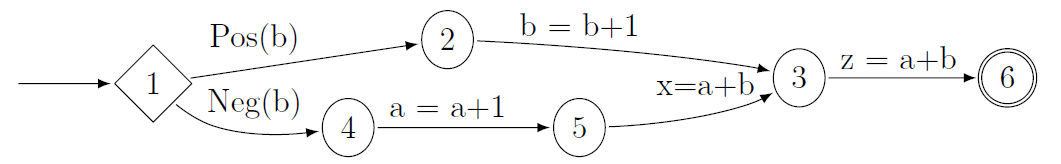
\includegraphics[width=\linewidth]{3org}\\
Transformed:\\
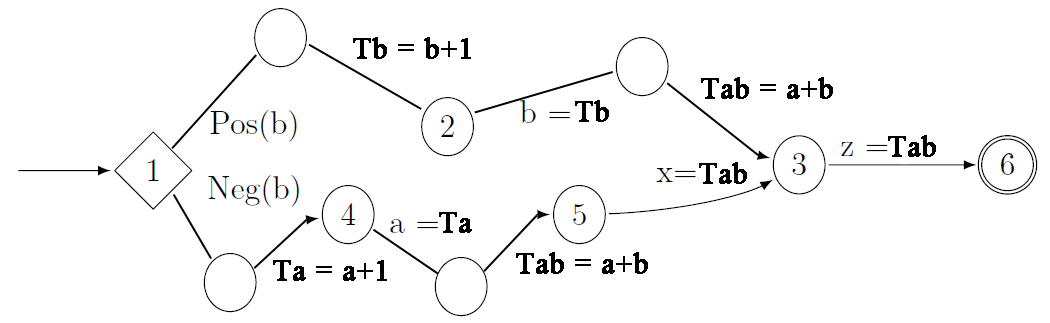
\includegraphics[width=\linewidth]{3}


\section*{Exercise 4: Loop rotation}
\subsection*{1. Pre-dominators}
\begin{tabular}{|c|c|}
\hline
 & $\mathcal{P}$ \\
\hline
1 & $\{1\}$ \\
2 & $\{1, 2\}$ \\
3 & $\{1, 2, 3\}$ \\
4 & $\{1, 2, 3, 4\}$ \\
5 & $\{1, 2, 3, 4, 5\}$ \\
6 & $\{1, 2, 6\}$ \\
\hline
\end{tabular}

\subsection*{2. Loop-rotation}
Original:\\
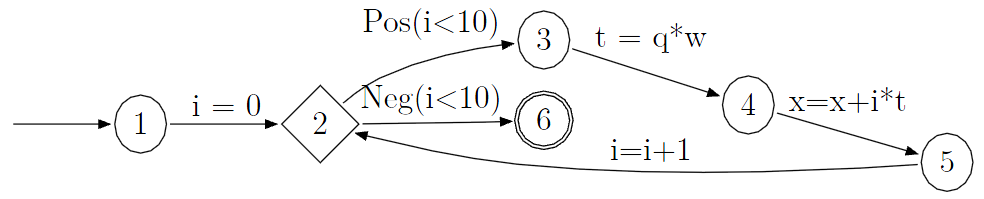
\includegraphics[width=\linewidth]{4org}\\
Transformed:\\
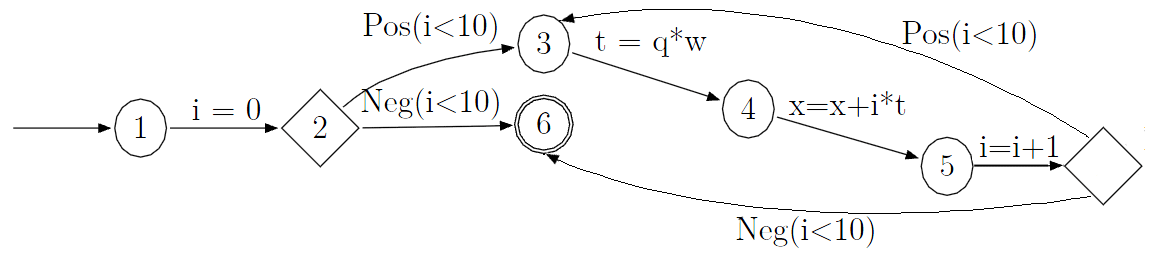
\includegraphics[width=\linewidth]{4}


\end{document}

















